\begin{frame}{}
    \begin{theorem}{ Erd\H{o}s--Szekeres theorem (1935)}
        Any sequence of \((n-1)(m-1)+1\) distinct real numbers contains either an increasing sequence of length \(n\) or a decreasing subsequence of length \(m\).
    \end{theorem}
    \pause
    \begin{proof}{Proof}
        \begin{columns}
        \begin{column}{0.75\linewidth}
        Label each number \(n_i\) in the sequence with the pair \((a_i,b_i)\)
        \begin{itemize}
            \item \(a_i\) - length of the longest increasing subsequence ending at \(n_i\)
            \item \(b_i\) - length of the longest decreasing subsequence ending at \(n_i\)
        \end{itemize}
        \pause
        Each \(n_i\) has a distinct pair \((a_i,b_i)\)\\
        \begin{itemize}
            \item if \(i<j\) and \(n_i<n_j\) then \(a_i<a_j\)
            \item if \(i<j\) and \(n_i>n_j\) then \(b_i<b_j\)
        \end{itemize}
        \end{column}
        \begin{column}{0.2\linewidth}
            \begin{figure}
                \centering
                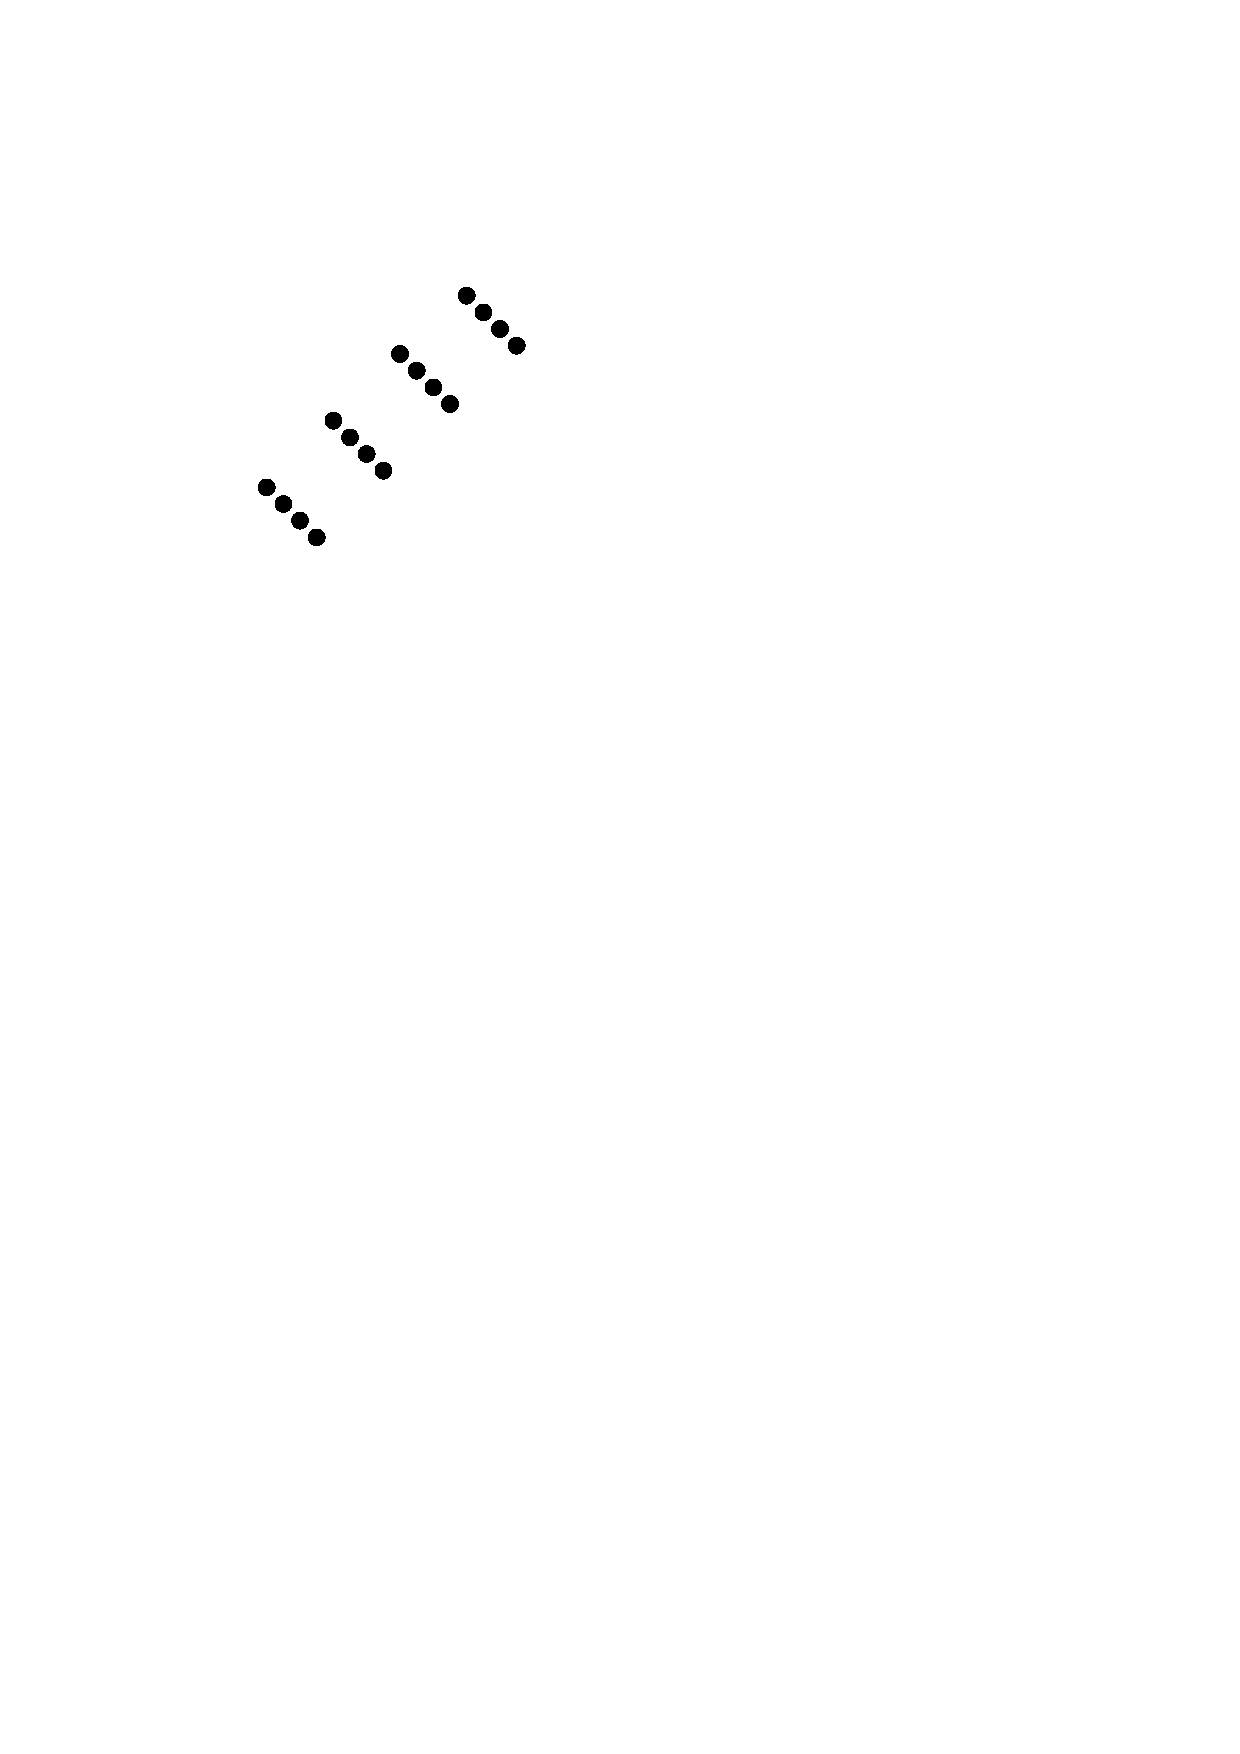
\includegraphics[width=0.8\linewidth]{images/esz.pdf}
            \end{figure}
        \end{column}
        \end{columns}
        \pause
        If \(a_i<n,b_i<m\) then there are at most \((n-1)(m-1)\) values, but there are \((n-1)(m-1)+1\) numbers thus contradiction.
    \end{proof}
\end{frame}

\begin{frame}
    % \begin{theorem}{Dilworth's Lemma}
    %     In any finite partially ordered set, the maximum size of an antichain equals the minimum number of chains needed to partition the set.
    % \end{theorem}
    \begin{theorem}{High-Order Monotonicity}
        A $(k+1)$-tuple is positive if its $k$-th derivative is nonnegative. A set is $k$-th order monotone if all its $(k+1)$-tuples are positive or all negative.
    \end{theorem}
    \begin{theorem}{Suk, 2017}
        Any $2^{n+o(n)}$ points in $\mathbb{R}^2$ contain a convex subset of size $n$.
    \end{theorem}
    \begin{theorem}{Xu, 2024}
        Any sequence of $n$ pairwise distinct real numbers contains a $k$-modal subsequence of length at least $\sqrt{(2k + 1)(n - \frac{1}{4})} - \frac{k}{2}$.
    \end{theorem}

\end{frame}

\begin{frame}{}
  \begin{ffact}{Array}
    A \textit{d-dimensional array} is an injective function
    \[
      f : A_1 \times \cdots \times A_d \to \mathbb{R},
    \]
    where \( A_1, \ldots, A_d \subseteq \mathbb{Z} \) are non-empty finite sets.
    We say \( f \) has size \( |A_1| \times \cdots \times |A_d| \).
  \end{ffact}
    \pause
  \medskip
  \begin{ffact}{Monotone Array}
    A \( d \)-dimensional array \( f \) is \textbf{monotone} if for each
    coordinate direction \( i \in [d] \), \emph{all} one-dimensional slices
    in direction \( i \) are increasing, \emph{or} all are decreasing.
  \end{ffact}
\end{frame}

\begin{frame}{Inconsistently Monotone Arrays}
  \begin{ffact}{Inconsistently monotone array}
    A \( d \)-dimensional array is \textbf{inconsistently monotone} if every
    one-dimensional slice is monotone (but slices along the same direction
    may go in different directions).
  \end{ffact}
\end{frame}


\begin{frame}{}
  \begin{ffact}{Lex--Monotone Array}
    A \( d \)-dimensional array \( f \) is \textbf{lex--monotone} if there exist
    a permutation \( \sigma : [d] \to [d] \) and signs \( s \in \{-1,+1\}^d \) such that
    \[
      f(x) < f(y) \;\iff\;
      \bigl(s_{\sigma(1)}\,x_{\sigma(1)},\ldots,s_{\sigma(d)}\,x_{\sigma(d)}\bigr)
      <_{\mathrm{lex}}
      \bigl(s_{\sigma(1)}\,y_{\sigma(1)},\ldots,s_{\sigma(d)}\,y_{\sigma(d)}\bigr).
    \]
  \end{ffact}
\end{frame}
\begin{frame}{Applications of lex--monotone arrays}
        \begin{hheading}{Poset dimension theory} lex--monotone arrays arise as realizers 
            of partial orders of bounded dimension
            \begin{itemize}
                \item Felsner, Fishburn, Trotter -- \textit{Finite three-dimensional partial 
                orders which are not sphere orders} (1999)
            \end{itemize}
        \end{hheading}
        \begin{hheading}{Temporal constraint satisfaction problem} lex--monotone structure 
            is used to determine the complexity of deciding temporal CSPs
            \begin{itemize}
                \item Bodirsky, K\'{a}ra -- \textit{The complexity of temporal constraint 
                satisfaction problems} (2010)
            \end{itemize}
        \end{hheading}
\end{frame}
\begin{frame}{}
    Our proofs work like:
    \vspace{-0.5cm}
\[
\text{Array} 
\rightarrow
\text{Inc. monotone}
\rightarrow
\text{Monotone}
\rightarrow
\text{Lex--monotone}
\]
\end{frame}